%%%%%%%%%%%%%%%%%%%%%%%%%%%%%%%%%%%%%%%
% Wenneker Resume/CV
% LaTeX Template
% Version 1.1 (19/6/2016)
%
% This template has been downloaded from:
% http://www.LaTeXTemplates.com
%
% Original author:
% Frits Wenneker (http://www.howtotex.com) with extensive modifications by 
% Vel (vel@LaTeXTemplates.com)
%
% License:
% CC BY-NC-SA 3.0 (http://creativecommons.org/licenses/by-nc-sa/3.0/
%
%%%%%%%%%%%%%%%%%%%%%%%%%%%%%%%%%%%%%%

%%%%%%%%%%%%%%%%%%%%%%%%%%%%%%%%%%%%%%
% David K Fehling Jr
% Updated: 04/06/2017
%%%%%%%%%%%%%%%%%%%%%%%%%%%%%%%%%%%%%%

%----------------------------------------------------------------------------------------
%	PACKAGES AND OTHER DOCUMENT CONFIGURATIONS
%----------------------------------------------------------------------------------------

\documentclass[a4paper,11pt]{memoir} % Font and paper size

%%%%%%%%%%%%%%%%%%%%%%%%%%%%%%%%%%%%%%%%%
% Wenneker Resume/CV
% Structure Specification File
% Version 1.1 (19/6/2016)
%
% This file has been downloaded from:
% http://www.LaTeXTemplates.com
%
% Original author:
% Frits Wenneker (http://www.howtotex.com) with extensive modifications by 
% Vel (vel@latextemplates.com)
%
% License:
% CC BY-NC-SA 3.0 (http://creativecommons.org/licenses/by-nc-sa/3.0/)
%
%%%%%%%%%%%%%%%%%%%%%%%%%%%%%%%%%%%%%%%%%
%
%Modified by: David Fehling (04/06/2017)
%
%%%%%%%%%%%%%%%%%%%%%%%%%%%%%%%%%%%%%%%%%

%----------------------------------------------------------------------------------------
%	PACKAGES AND OTHER DOCUMENT CONFIGURATIONS
%----------------------------------------------------------------------------------------

\usepackage{XCharter} % Use the Bitstream Charter font
\usepackage[utf8]{inputenc} % Required for inputting international characters
\usepackage[T1]{fontenc} % Output font encoding for international characters

\usepackage[top=1cm,left=1cm,right=1cm,bottom=1cm]{geometry} % Modify margins

\usepackage{graphicx} % Required for figures

\usepackage{flowfram} % Required for the multi-column layout

\usepackage{url} % URLs

\usepackage[usenames,dvipsnames]{xcolor} % Required for custom colours

\usepackage{tikz} % Required for the horizontal rule

\usepackage{enumitem} % Required for modifying lists
\setlist{noitemsep,nolistsep} % Remove spacing within and around lists

\setlength{\columnsep}{\baselineskip} % Set the spacing between columns

% Define the left frame (sidebar)
\newflowframe{0.15\textwidth}{\textheight}{0pt}{0pt}[left]
\newlength{\LeftMainSep}
\setlength{\LeftMainSep}{0.15\textwidth}
\addtolength{\LeftMainSep}{1\columnsep}
 
% Small static frame for the vertical line
\newstaticframe{1.5pt}{\textheight}{\LeftMainSep}{0pt}
 
% Content of the static frame with the vertical line
\begin{staticcontents}{1}
\hfill
\tikz{\draw[loosely dotted,color=RoyalBlue,line width=1.5pt,yshift=0](0,0) -- (0,\textheight);}
\hfill\mbox{}
\end{staticcontents}
 
% Define the right frame (main body)
\addtolength{\LeftMainSep}{1.5pt}
\addtolength{\LeftMainSep}{1\columnsep}
\newflowframe{0.7\textwidth}{\textheight}{\LeftMainSep}{0pt}[main01]

\pagestyle{empty} % Disable all page numbering

\setlength{\parindent}{0pt} % Stop paragraph indentation

%----------------------------------------------------------------------------------------
%	NEW COMMANDS
%----------------------------------------------------------------------------------------

\newcommand{\userinformation}[1]{\renewcommand{\userinformation}{#1}} % Define a new command for the CV user's information that goes into the left column

\newcommand{\cvheading}[1]{{\Huge\bfseries\color{RoyalBlue} #1} \par\vspace{.6\baselineskip}} % New command for the CV heading
\newcommand{\cvsubheading}[1]{{\Large\bfseries #1} \bigbreak} % New command for the CV subheading

\newcommand{\Sep}{\vspace{1em}} % New command for the spacing between headings
\newcommand{\SmallSep}{\vspace{0.5em}} % New command for the spacing within headings

\newcommand{\aboutme}[2]{ % New command for the about me section
\textbf{\color{RoyalBlue} #1}~~#2\par\Sep
}
	
\newcommand{\CVSection}[1]{ % New command for the headings within sections
{\Large\textbf{#1}}\par
\SmallSep % Used for spacing
}

\newcommand{\CVItem}[2]{ % New command for the item descriptions
\textbf{\color{RoyalBlue} #1}\par
#2
\SmallSep % Used for spacing
}

\newcommand{\bluebullet}{\textcolor{RoyalBlue}{$\circ$}~~} % New command for the blue bullets
 % Include the file specifying document layout and packages

%----------------------------------------------------------------------------------------
%	NAME AND CONTACT INFORMATION 
%----------------------------------------------------------------------------------------

\userinformation{ % Set the content that goes into the sidebar of each page
\begin{flushright}
% Comment out this figure block if you don't want a photo
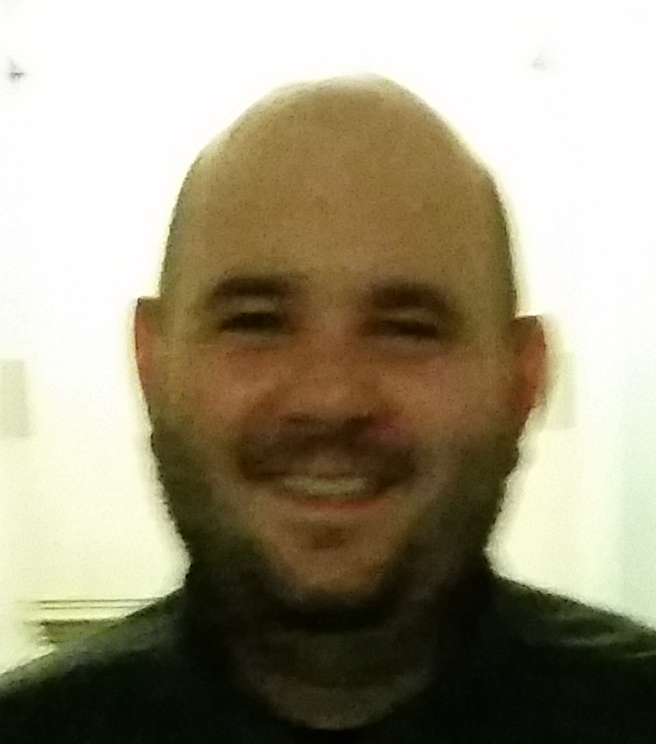
\includegraphics[width=0.6\columnwidth]{portrait_crop.jpg}\\[\baselineskip] % Your photo
\small % Smaller font size
\textbf{David Fehling} \\ % Your name
\Sep
\quad\url{dfehling@gmail.com} \\ % Your email address
\Sep
\url{github.com/dfehling} \\ % Your URL
\Sep
(443) 761-8728 \\ % Your phone number
\Sep % Some whitespace
\textbf{Address} \\
8943 Sahalee Ct \\ % Address 1
Pasadena, MD 21122 \\ % Address 2
% Country \\ % Address 3
\vfill % Whitespace under this block to push it up under the photo
\end{flushright}
}

%----------------------------------------------------------------------------------------

\begin{document}

\userinformation % Print your information in the left column

\framebreak % End of the first column

%----------------------------------------------------------------------------------------
%	HEADING
%----------------------------------------------------------------------------------------

\cvheading{David Fehling} % Large heading - your name

\cvsubheading{Data Scientist} % Subheading - your occupation/specialization

%----------------------------------------------------------------------------------------
%	ABOUT ME
%----------------------------------------------------------------------------------------
\CVSection{Overview}
\aboutme{}{I am a Ph.D Physicist with data analysis experience seeking a data scientist role. As a member of the CMS Collaboration at CERN, I analyzed large datasets using statistical methods. This analysis was done both independently and collaboratively, and the results were presented to internal and external groups. I have demonstrated a comprehensive leadership role in educating students regarding both general physics and experimental high energy physics research.}


%----------------------------------------------------------------------------------------
%   EXPERIENCE
%----------------------------------------------------------------------------------------

\CVSection{Personal Experience}

\CVItem{August 2014 - December 2016, \textit{Research Assistant and Data Analyst}, Johns Hopkins University}{
\begin{itemize}
    \item Worked independently and collaboratively on data analysis
    \item Presented results of analysis to small groups
    \item Wrote code used by 3000-member collaboration
    \item Worked with large datasets (>1 PB)
    % \item Awarded E.J. Rhee Teaching Award for 2015
    \item Responsible for Teaching Assistants (TAs) as Head Laboratory TA
\end{itemize}
}

\CVItem{March 2012 - August 2014, \textit{Representative, Inbound Sales and Support}, GoDaddy}{
\begin{itemize}
    \item Provided technical support for customers
    \item Consulted with customers about how to grow their online businesses
    \item Consistently exceeded sales goals and quality metrics
    \item Quickly rose to leadership role on top sales team
\end{itemize}
}

%------------------------------------------------

\Sep % Extra whitespace after the end of a major section

%----------------------------------------------------------------------------------------
%	EDUCATION
%----------------------------------------------------------------------------------------

\CVSection{Education}

%------------------------------------------------

\CVItem{2016 - Ph.D, Physics\quad\quad\quad\quad\quad2012 - M.A., Physics}{Johns Hopkins University}

\CVItem{2005 - B.S., Physics\quad\quad\quad\quad\quad~2005 - B.S., Chemistry}{University of West Florida}

%------------------------------------------------

\Sep % Extra whitespace after the end of a major section


%----------------------------------------------------------------------------------------
%   SKILLS
%----------------------------------------------------------------------------------------

\CVSection{Analysis Skills}
%------------------------------------------------

\CVItem{Programming}
{\begin{tabular}{p{0.23\textwidth} p{0.23\textwidth} p{0.23\textwidth}}
\bluebullet C++ &  \bluebullet Python & \bluebullet R \\
\bluebullet Roofit &  \bluebullet SQL & \\
\end{tabular}}
%------------------------------------------------

%------------------------------------------------
%For some reason I need these to end the previous table
% \framebreak
% \Sep
% \\
% \framebreak

\CVItem{Statistical Background}
{\begin{tabular}{p{0.23\textwidth} p{0.23\textwidth} p{0.23\textwidth}}
\bluebullet Numerical Methods &  \bluebullet Error Analysis & \bluebullet Model Building \\
\bluebullet Linear Regression &  \bluebullet Monte Carlo Methods & \bluebullet Likelihood Analysis \\
% \bluebullet Linear Regression &  \bluebullet Monte Carlo Methods & \bluebullet Probability Distributions \\
\end{tabular}}

\CVItem{Mathematical Background}
{\begin{tabular}{p{0.3\textwidth} p{0.3\textwidth}}
\bluebullet Multivariate Calculus &  \bluebullet Linear Algebra \\
\bluebullet Matrix Factorization & \bluebullet Fourier Analysis \\
\end{tabular}}

%------------------------------------------------

\Sep % Extra whitespace after the end of a major section

%----------------------------------------------------------------------------------------
%	NEW PAGE DELIMITER
%	Place this block wherever you would like the content of your CV to go onto the next page
%----------------------------------------------------------------------------------------

% \clearpage % Start a new page

% \userinformation % Print your information in the left column

% \framebreak % End of the first column

%----------------------------------------------------------------------------------------
%	AWARDS
%----------------------------------------------------------------------------------------

% \CVSection{Awards}

% %------------------------------------------------

\CVSection{Accomplishments}
Led international tours of CMS detector at the LHC in France\\
Exhibitor at the US Science and Engineering Expo (2014,2016)\\
Awarded E.J. Rhee Teaching Award in 2015\\

\Sep % Extra whitespace after the end of a major section

%----------------------------------------------------------------------------------------

\end{document}
